\documentclass[12pt,a4paper,oneside,ngerman]{article} 
\usepackage[left=3cm,right=3cm,top=2.5cm]{geometry} % Groesse der Seitenraender definieren
\usepackage[utf8]{inputenc} % utf8 encoding
\usepackage{hyperref}
\usepackage{ngerman}
\usepackage{graphicx}
\graphicspath{{Von Pieter/}}
\usepackage{tikz} % Automaten, Graphen, ... zeichnen
\usepackage{tikz-qtree} % Paket fuer Tikz Graphen-Baeume
\usetikzlibrary{arrows,shapes,automata} % Bestimmte tikz-Befehle benutzen
\usepackage{amsmath,amssymb} % Mathe-Formeln und -Ausdruecke
\usepackage{listings} % Code-Ausschnitte einbinden
\usepackage{xcolor} % Eigene Farben definieren
\usepackage{colortbl} % Farben verwenden in Tabellen
\usepackage{wrapfig} % Bilder von Text umfliessen lassen
\usepackage{multicol} % Mehrspaltigen Text schreiben
\usepackage{stmaryrd} % Fuer Symbole wie zu Beispiel Widerspruchspfeil
\usepackage{caption}
\usepackage{totpages}

%Java Code für listing definiert
\lstset{language=Java,
basicstyle=\small \ttfamily,
keywordstyle=\color{javapurple}\bfseries,
stringstyle=\color{javared},
commentstyle=\color{javagreen},
morecomment=[s][\color{javadocblue}]{/**}{*/},
numbers=left,
numberstyle=\tiny\color{black},
stepnumber=1,
numbersep=10pt,
tabsize=1,
showspaces=false,
showstringspaces=false,
breaklines}
\lstset{literate=%
  {Ö}{{\"O}}1
  {Ä}{{\"A}}1
  {Ü}{{\"U}}1
  {ß}{{\ss}}1
  {ü}{{\"u}}1
  {ä}{{\"a}}1
  {ö}{{\"o}}1
}

% Beliebige RGB Farben definieren:
\definecolor{gold}{rgb}{0.83, 0.69, 0.15}
\definecolor{magenta}{rgb}{0.79, 0.08, 0.48}
\definecolor{javared}{rgb}{0.6,0,0} % for strings
\definecolor{javagreen}{rgb}{0.25,0.5,0.35} % comments
\definecolor{javapurple}{rgb}{0.5,0,0.35} % keywords
\definecolor{javadocblue}{rgb}{0.25,0.35,0.75} % javadoc

% Titel in Kopfzeilen
\usepackage{fancyhdr}
\pagestyle{fancy}
\fancyhf{}
\setlength{\headheight}{20pt}

% Seitenumbrueche werden nicht mehr eingerueckt
\setlength{\parindent}{0em}


% % % % % % % % % % % % % % % % % % % % % % % % % % % % % % 
%Variablen
% % % % % % % % % % % % % % % % % % % % % % % % % % % % % % 
\newcommand{\fach}{Objektorientierte Modellierung und Programmierung}
\newcommand{\dokumentenTitel}{Abgabe Uebungsblatt Nr.02}
\newcommand{\Abgabe}{05.05.2020, 12:00 Uhr}
\newcommand{\memberOne}{Marius Birk}
\newcommand{\memberTwo}{Pieter Vogt}


\newcommand{\tutor}{ Florian Brandt }
% % % % % % % % % % % % % % % % % % % % % % % % % % % % % 

% Kopfzeile auf jeder Seite:
\fancyhead[R]{\dokumentenTitel} % Dokument-Titel
\fancyhead[C]{}
\fancyhead[L]{\memberOne, \memberTwo} % Autorennamen
\renewcommand{\headrulewidth}{0.4pt} %obere Trennlinie

% Fußzeile auf jeder Seite:
\fancyfoot[C]{Seite \thepage \ von \ref{TotPages}} %Seitennummer
\renewcommand{\footrulewidth}{0.4pt} %untere Trennlinie

% Nun beginnt das eigentliche Dokument
\begin{document}
	\thispagestyle{plain} % Keine Kopfzeile auf erster Seite, aber Seitenzahl wird angezeigt
	
	\begin{multicols}{2} % Beginnt zweispaltigen Text fuer Header auf erster Seite
		\hspace{-1cm} % Linken Header-Teil 1cm nach links schieben.
		% Tabelle fuer linke Seite vom Header der ersten Seite
		\begin{tabular}{ll} % Mit l werden die Eintraege linksbuendig
			Autoren: & \memberOne \\ % Zwischen jeder Spalte ein & einfuegen
			& \memberTwo \\
% beendet eine Tabellenzeile 
			Tutor: & \tutor \\  
		\end{tabular}
		
		\columnbreak % Nun beginnt die rechte Seite des Headers
		\hspace{-1cm} % Rechten Header-Teil 1cm nach links schieben.
		% Tabelle fuer rechte Seite vom Header der ersten Seite
		\begin{tabular}{ll} % p{1cm} bewirkt, dass die rechte Spalte 6cm breit ist.
			Abgabe: & \Abgabe \\ % Zwischen jeder Spalte ein & einfuege
			Smileys: &  
			%Mit diesem Befehl wird die Zeilenhoehe der folgenden Tabelle um 20% erhoeht.   
			\renewcommand{\arraystretch}{1.2} 
			% Nun kommt eine innere Tabelle in der aeusseren Tabelle, mit der eine Punktetabelle fuer den Tutor erstellt wird:  
			\begin{tabular}{|p{0.8cm}|p{0.8cm}|p{0.8cm}|p{0.8cm}|}
				\hline A1 & A2 & A3 & $\sum\limits^{ }$ \\ \hline
				& & & \\ \hline    
			\end{tabular} \\
		\end{tabular}
		
	\end{multicols} % Beendet zweispaltigen Text
	
	\begin{center}
		\Large{\fach} \\
		\LARGE{\dokumentenTitel} \\
		\small
		$($Alle allgemeinen Definitionen aus der Vorlesung haben in diesem Dokument bestand, es sei den sie erhalten eine explizit andere Definition.$)$
    \end{center}


	\section{Aufgabe 1}


\begin{figure}[ht]
	\centering
	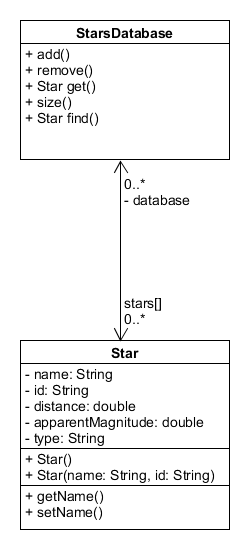
\includegraphics[scale=0.5]{Klassendiagramm Sternendatenbank}
	\caption{Klassendiagramm der Sternendatenbank}
	\label{fig1}
\end{figure}

\begin{figure}[ht]
	\centering
	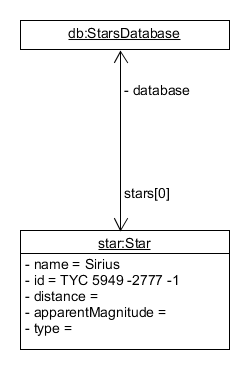
\includegraphics[scale=0.5]{Objektdiagramm Test1 Sternendatenbank}
	\caption{Objektdiagramm: Test 1}
	\label{fig2}
\end{figure}

\begin{figure}[ht]
	\centering
	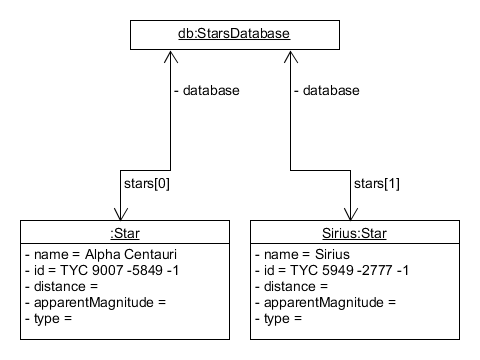
\includegraphics[scale=0.5]{Objektdiagramm Test2 Sternendatenbank}
	\caption{Objektdiagramm: Test 2}
	\label{fig3}
\end{figure}

\begin{figure}[ht]
	\centering
	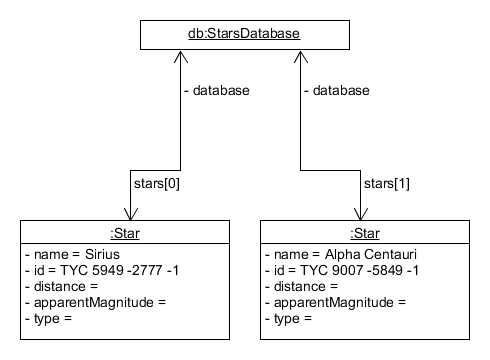
\includegraphics[scale=0.5]{Objektdiagramm Test3 Sternendatenbank}
	\caption{Objektdiagramm: Test 3}
	\label{fig4}
\end{figure}



	
    \section{Aufgabe 2}
        \subsection{a)}
            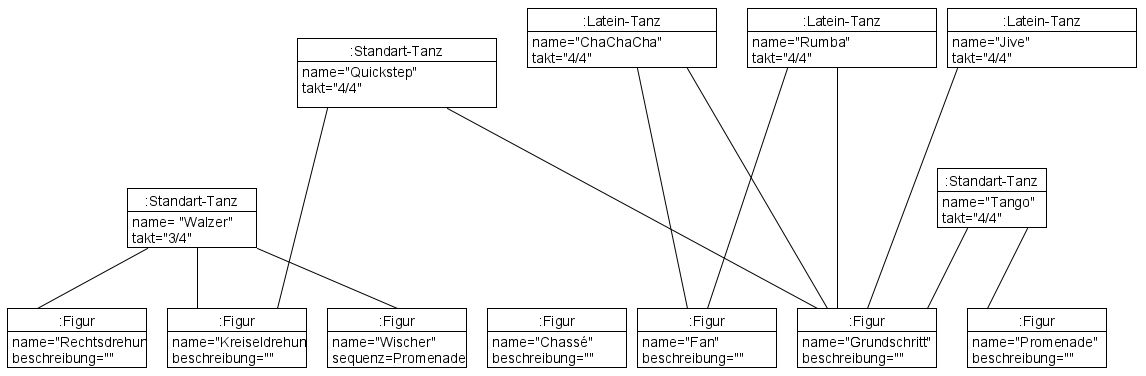
\includegraphics[width=18cm]{Objektdiagramm A_2}\\\\
        \subsection{b)}
                \subsubsection{Dance Code}
                    \begin{verbatim}
						import java.util.ArrayList;
						class Dance {
							private String name;
							private String beat;
							private Object[] figures = new Object[3];
						
							public Object[] getFigures() {
								return figures;
							}
						
							public void setFigures(Object[] figures) {
								for(int i = 0; i< figures.length; i++){
									this.figures[i] = figures[i];
								}
							}
						
							public String getName() {
								return name;
							}
						
							public void setName(String name) {
								this.name = name;
							}
						
							public String getBeat() {
								return beat;
							}
						
							public void setBeat(String beat) {
								this.beat = beat;
							}
						}
						class StandardDance extends Dance{
						
						}
						class LatinDance extends Dance{
						
						}
						class Figure{
							private String name;
							private String text;
						
							public String getName() {
								return name;
							}
						
							public void setName(String name) {
								this.name = name;
							}
						
							public String getText() {
								return text;
							}
						
							public void setText(String text) {
								this.text = text;
							}
						}
						class Sequence extends Figure{
							private String name;
							public ArrayList<Object> figures = new ArrayList<Object>();
							public void setSequence(ArrayList sequence){
								this.figures = sequence;
							}
							public boolean add(Figure figure){
								if( figure instanceof Sequence){
									return false;
								}
								else{
									figures.add(figure);
									return true;
								}
							}
						}
					\end{verbatim}
				\subsubsection{Dance Database}
					\begin{verbatim}
						import java.io.FileReader;
import java.lang.reflect.Array;
import java.util.ArrayList;

public class DanceDatabase {
    public static void main(String[] args) {
        Figure Righturn = new Figure();
        Righturn.setName("Rightturn");
        Righturn.setText("Turning right");

        Figure Circle = new Figure();
        Circle.setName("Circle");
        Circle.setText("Circle");

        Figure Whisk = new Figure();
        Whisk.setName("Whisk");

        Figure Chasse = new Figure();
        Chasse.setName("Chassé");
        Chasse.setText("Chassé");

        Figure Fan = new Figure();
        Fan.setText("Fan");
        Fan.setName("Fan");

        Figure Basic = new Figure();
        Basic.setName("Basic Movement");
        Basic.setText("Basic Movement");

        Figure Promenade = new Figure();
        Promenade.setText("Promenade");
        Promenade.setName("Promenade");

        Sequence S_Whisk = new Sequence();
        if(S_Whisk.add(Chasse)){
            System.out.println("Hinzufügen erfolgreich");
            //Um diese Prüfung zu realisieren musste das Objekt Array auf eine Object ArrayList geändert werden, in dem die Figuren
            //gespeichert werden.
        }
        else{
            System.out.println("Hinzufügen nicht erfolgreich");

        }
        StandardDance Walzer = new StandardDance();
        Walzer.setName("Walzer");
        Walzer.setBeat("3/4");
        Object[] figures = new Object[]{Righturn, Circle, Whisk};
        Walzer.setFigures(figures);
        figures = null;

        StandardDance Tango = new StandardDance();
        Tango.setBeat("4/4");
        Tango.setName("Tango");
        figures= new Object[]{Basic, Promenade};
        Tango.setFigures(figures);
        figures= null;

        StandardDance Quickstep = new StandardDance();
        Tango.setBeat("4/4");
        Tango.setName("Quickstep");
        figures = new Object[]{Basic, Circle};
        Tango.setFigures(figures);
        figures= null;

        LatinDance Cha = new LatinDance();
        Cha.setBeat("4/4");
        Cha.setName("ChaChaCha");
        figures = new Object[]{Basic, Fan};
        Cha.setFigures(figures);
        figures= null;

        LatinDance Rumba = new LatinDance();
        Rumba.setBeat("4/4");
        Rumba.setName("Rumba");
        figures = new Object[]{Basic, Fan};
        Cha.setFigures(figures);
        figures= null;

        LatinDance Jive = new LatinDance();
        Jive.setBeat("4/4");
        Jive.setName("ChaChaCha");
        figures = new Object[]{Basic};
        Jive.setFigures(figures);
        figures= null;
    }
}

					\end{verbatim}
			\subsection{c)}
			\begin{verbatim}
				public boolean add(Figure figure){
        if( figure instanceof Sequence){
            return false;
        }
        else{
            figures.add(figure);
            return true;
        }
    }
			\end{verbatim}
	\section{Aufgabe 3}
			\subsection{a)}

\begin{lstlisting}
public class Out {

   public static void out(boolean bool) {
      System.out.println(bool);
   }

   public static void out(int number) {
      System.out.println(number);
   }

   public static void out(double number) {
      System.out.println(number);
   }

   public static void out(char character) {
      System.out.println(character);
   }

   public static void out(String string) {
      System.out.println(string);
   }

   public static void out(Object obj) {
      System.out.println(obj);
   }

}
\end{lstlisting}

\end{document}
